\documentclass[letterpaper]{report}
\usepackage[T1]{fontenc}
\usepackage{RJournal}
\usepackage{amsmath,amssymb,array,booktabs}
\usepackage[spanish,es-noshorthands]{babel}
\usepackage{graphicx}
\usepackage{fancyvrb}
\graphicspath{{../../outputs/R/figuras/}{../../outputs/julia/figuras/}}
\renewcommand{\abstract}[1]{\setstretch{1}\noindent\small\textbf{Resumen.} #1}
\providecommand{\keywords}[1]{\par\smallskip\noindent\small\textbf{Palabras clave:} #1\par}
\hypersetup{pdfauthor={Rodrigo Claudio Rosas Tuni}}
\begin{document}
\sectionhead{Analítica prescriptiva con R}
\year{2026}
\begin{article}
\title{Analítica prescriptiva del rendimiento de papa en el Perú con R: del pronóstico con historial reducido a la asignación óptima de inversión (ENA 2015--2025)}
\author{Rodrigo Claudio Rosas Tuni}
\maketitle
\abstract{La Encuesta Nacional Agropecuaria (ENA) deja solo diez años útiles para la papa (2015--2025, sin 2020). Este trabajo lleva el pronóstico con historial reducido de un artículo previo a una pregunta de decisión: con S/ 50 millones por campaña, ¿en qué departamentos y en qué palancas conviene invertir? El pipeline, escrito en R con \pkg{tidyverse}, \pkg{caret}, \pkg{easystats}, \pkg{xgboost}, \pkg{lpSolve}, \pkg{shiny} y \pkg{shinytest2}, tiene seis ramas y 61 validaciones automáticas. Primero reconstruye el panel departamental desde los microdatos y reproduce el artículo: el ensamble informado logra un RMSE de 3\,092.66 kg/ha frente a 3\,361.84 del modelo ingenuo, y la calibración conformal lleva la cobertura del 80\,\% nominal de 50.5\,\% a 81.1\,\%. Después estima el efecto de cada palanca con efectos fijos y resuelve un programa lineal con restricciones de presupuesto, topes y equidad para los 6 departamentos con heladas frecuentes. El plan robusto, que usa la cota inferior de los efectos, destina 65\,\% del presupuesto a los departamentos priorizados, sobre todo en semilla certificada, y produce un valor adicional de S/ 131.7 millones con una probabilidad de no recuperar la inversión de 0.59\,\%.}
\keywords{analítica prescriptiva - programación lineal - calibración conformal - papa - R}

\section{1. Introducción y reto}
En un trabajo previo del grupo \citep{articulo} se pronosticó el rendimiento de papa de la ENA \citep{inei} con el marco de \citet{huang} para historial reducido: covariables de dominio, validación rolling-origin y calibración conformal. Ese trabajo responde a la pregunta \emph{qué va a pasar}. Para una institución pública la pregunta útil es otra: \emph{qué hacer con un presupuesto limitado}. Esa es la tarea de la analítica prescriptiva.

\textbf{Reto.} Con S/ 50 millones por campaña, decidir cuánto subir cuatro palancas (riego tecnificado, semilla certificada, asistencia técnica y crédito) en 19 departamentos para obtener el mayor valor de producción adicional, sin concentrar el gasto y sin dejar de lado a los departamentos con heladas frecuentes. El pipeline debe ser reproducible, validarse a sí mismo y comunicar la decisión a quien no programa.

El trabajo se preparó para LatinR. Este informe documenta la versión en R; un informe gemelo hace lo mismo en Julia \citep{julia} y ambos comparan sus resultados.

\section{2. Rama 0: ruta del pipeline}
Todas las rutas se definen una sola vez en el archivo de configuración y se construyen desde la raíz del proyecto, de modo que el código funciona en cualquier computadora. Los insumos son tres archivos: \code{ENA\_cultivo\_filas.csv} (139\,466 filas de papa cosechada), \code{ENA\_productores.csv} (384\,525 productores) y \code{series\_ENA\_papa.xlsx} (series agregadas). Cada uno tiene una huella SHA-256 registrada: si un archivo cambia, el pipeline se detiene en la primera línea. El Cuadro~\ref{tab:ramas} resume las seis ramas.

\begin{table}[htbp]
\centering\small
\caption{Ramas del pipeline y producto de cada una.}\label{tab:ramas}
\begin{tabular}{p{0.9cm}p{4.2cm}p{9.8cm}}
\toprule
Rama & Archivo & Qué hace \\
\midrule
0 & \code{00\_config.R} & Rutas de datos, huellas SHA-256 y todos los parámetros (modelo y supuestos). \\
1 & \code{01\_librerias.R} & Verifica e importa las librerías; registra versiones. \\
2 & \code{02\_datos\_validacion.R} & Reconstruye el panel desde los microdatos y lo contrasta con el Excel. \\
3 & \code{03\_descriptivo\_easystats.R} & Descriptivos, correlaciones y modelo de efectos fijos con diagnóstico \pkg{easystats}. \\
4 & \code{04\_predictivo\_walkforward.R} & Réplica del artículo: walk-forward, conformal, heladas, SHAP; verificación con \pkg{caret}. \\
5 & \code{05\_prescriptivo.R} & Alerta 2026, efectos de palancas, programa lineal, Montecarlo y frontera. \\
6 & \code{06\_comunicacion\_pruebas.R} & Tablero \pkg{shiny}, pruebas \pkg{testthat}/\pkg{shinytest2} y registro final. \\
\bottomrule
\end{tabular}
\end{table}
\begin{Verbatim}[fontsize=\scriptsize, frame=single, framesep=2mm, label={\small Estructura de carpetas}]
ENA_papa_prescriptivo/
  data/raw/          insumos (solo lectura)
  data/referencia/   métricas y pronósticos del artículo (Python)
  R/                 ramas 00-06, funciones, app/ (Shiny) y tests/
  julia/             ramas 00-06, funciones y test/
  outputs/R | julia/ tablas/, figuras/, logs y resumen JSON
  informes/          fuentes LaTeX de este informe
\end{Verbatim}
\section{3. Rama 1: librerías}
Se usan las librerías pedidas para el trabajo: \pkg{tidyverse} \citep{tidyverse} para datos y gráficos, \pkg{caret} \citep{caret} como interfaz de modelos, \pkg{easystats} \citep{easystats} para diagnóstico y reporte, y \pkg{shinytest2} para probar el tablero. El Cuadro~\ref{tab:libs} indica el papel de cada una. El análisis corrió en R 4.5.3.

\begin{table}[htbp]
\centering\small
\caption{Librerías de R usadas y su papel en el pipeline.}\label{tab:libs}
\begin{tabular}{p{3.2cm}p{1.6cm}p{10cm}}
\toprule
Librería & Versión & Uso \\
\midrule
\pkg{tidyverse} & 2.0.0 & Lectura (\pkg{readr}), agregación ponderada (\pkg{dplyr}), pivotes y figuras (\pkg{ggplot2}). \\
\pkg{caret} & 7.0.1 & Verificación del panel FE-ARDL con índices walk-forward propios en \code{trainControl()}. \\
\pkg{easystats} & 0.7.6 & \pkg{correlation}, \pkg{parameters} (errores agrupados), \pkg{performance} (diagnósticos) y \pkg{see}. \\
\pkg{xgboost} & 3.4.2.1 & Árbol restringido (profundidad 2) y valores SHAP exactos con \code{predcontrib = TRUE}. \\
\pkg{glmnet} & 5.0 & Disponible para contraste; ElasticNet se implementa con la función objetivo de scikit-learn. \\
\pkg{sandwich} & 3.1.3 & Matriz de covarianza agrupada por departamento (CR1). \\
\pkg{lpSolve} & 5.6.23 & Programa lineal de la analítica prescriptiva, con precios sombra. \\
\pkg{shiny} & 1.14.0 & Tablero interactivo para quien decide. \\
\pkg{shinytest2} & 0.6.0 & Prueba de extremo a extremo del tablero en Chrome. \\
\pkg{testthat} & 3.3.2 & Pruebas unitarias y de servidor (\code{testServer}). \\
\pkg{digest} & 0.6.39 & Huellas SHA-256 de los archivos de entrada. \\
\bottomrule
\end{tabular}
\end{table}
\section{4. Rama 2: datos y validación}
Antes de modelar se rehízo el panel departamental desde los microdatos: el rendimiento es $\sum f_k\,\mathrm{kg}_k/\sum f_k\,\mathrm{ha}_k$ con el factor de expansión $f_k$, y cada covariable es un porcentaje ponderado entre quienes respondieron. En la ENA 2025 el módulo de pérdidas solo lista a quienes perdieron, así que el resto se cuenta como sin pérdida. Las 196 celdas año-departamento coinciden con el Excel en las 14 variables (diferencia máxima 5.8e-11). Hay 142 filas válidas sin ubigeo (2024--2025): entran a la serie nacional, pero no a ningún departamento.

El panel de análisis tiene 19 departamentos con los 10 años (Loreto y San Martín quedan fuera por tener solo tres). El crédito de 2021 no se preguntó; se arrastra el valor de 2019 del mismo departamento, que es información pasada. Cada regla anterior es una validación que detiene el pipeline si falla:

\begin{Verbatim}[fontsize=\scriptsize, frame=single, framesep=2mm, label={\small Función de validación (se usa en todas las ramas)}]
chequear <- function(rama, prueba, condicion, detalle = "") {
  ok <- isTRUE(all(condicion))
  VALIDACIONES <<- add_row(VALIDACIONES, rama = rama, prueba = prueba, ok = ok, detalle = as.character(detalle))
  if (!ok) stop(sprintf("[VALIDACIÓN FALLIDA] %s - %s %s", rama, prueba, detalle), call. = FALSE)
  invisible(ok)
}
\end{Verbatim}
\section{5. Rama 3: descriptivo y diagnóstico}
Las medias por departamento reproducen el Cuadro~1 del artículo al centésimo: la costa (Lima, Ica, Arequipa) supera los 20\,000 kg/ha y Puno y Lambayeque no llegan a 6\,100 (Figura~\ref{fig:evol}). Las correlaciones con el rendimiento también coinciden: crédito (0.55), semilla certificada (0.49), riego (0.45) y asistencia técnica (0.41). Son correlaciones entre departamentos; para decidir hace falta saber qué pasa \emph{dentro} de un mismo departamento cuando una palanca sube.

\begin{figure}[htbp]
\centering
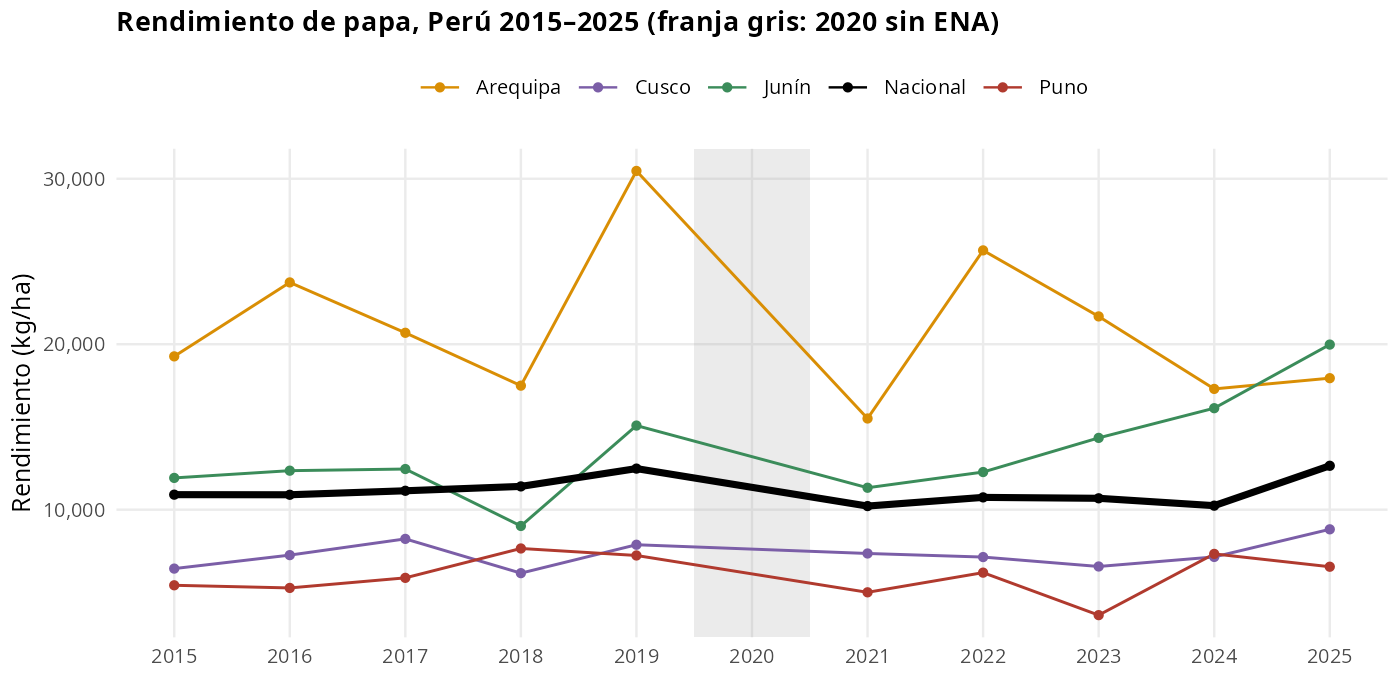
\includegraphics[width=0.85\textwidth]{r01_evolucion.png}
\caption{Rendimiento nacional y de cuatro departamentos, 2015--2025.}\label{fig:evol}
\end{figure}
Por eso la prescripción se apoya en un modelo con efectos fijos por departamento y por año (Cuadro~\ref{tab:ef}). Los efectos fijos absorben lo que no cambia en cada departamento (altitud, suelos, costa o sierra) y los choques comunes de cada año. El diagnóstico muestra heterocedasticidad fuerte (Breusch--Pagan, $p = 1.2e-34$) y residuos no normales (Shapiro--Wilk, $p = 3.6e-09$); el VIF máximo es 2.46, sin colinealidad preocupante. Esto justifica los errores agrupados por departamento y, más adelante, los intervalos conformales.

\begin{table}[htbp]
\centering
\small
\caption{Modelo explicativo con efectos fijos por departamento y año (190 obs.). Errores estándar agrupados por departamento (CR1).}\label{tab:ef}
\begin{tabular}{lrrrr}
\toprule
Covariable (pp) & $\hat\beta$ (kg/ha) & EE agrupado & $t$ & $p$ \\
\midrule
Riego (\% área) & 4.1 & 29.0 & 0.14 & 0.889 \\
Semilla certificada (\% área) & 70.5 & 18.0 & 3.91 & 0.000 \\
Fertilizante & 16.7 & 28.6 & 0.58 & 0.561 \\
Abono & 62.8 & 23.7 & 2.65 & 0.009 \\
Asistencia técnica & 101.0 & 65.8 & 1.54 & 0.127 \\
Capacitación & -41.7 & 34.5 & -1.21 & 0.229 \\
Asociatividad & -10.7 & 59.7 & -0.18 & 0.858 \\
Crédito & 43.7 & 52.5 & 0.83 & 0.406 \\
Pérdida por helada & -24.3 & 42.7 & -0.57 & 0.570 \\
Pérdida por sequía & 216.1 & 104.1 & 2.08 & 0.039 \\
\bottomrule
\end{tabular}
\end{table}
Dentro de cada departamento, un punto porcentual más de área con semilla certificada se asocia con 70.5 kg/ha más ($p = 0.0001$). La asistencia técnica tiene un coeficiente mayor (101.0) pero impreciso ($p = 0.13$). El riego, muy correlacionado entre departamentos, casi no se mueve dentro de ellos (4.1 kg/ha, $p = 0.89$): en diez años un departamento cambia poco su superficie regada.

\begin{figure}[htbp]
\centering
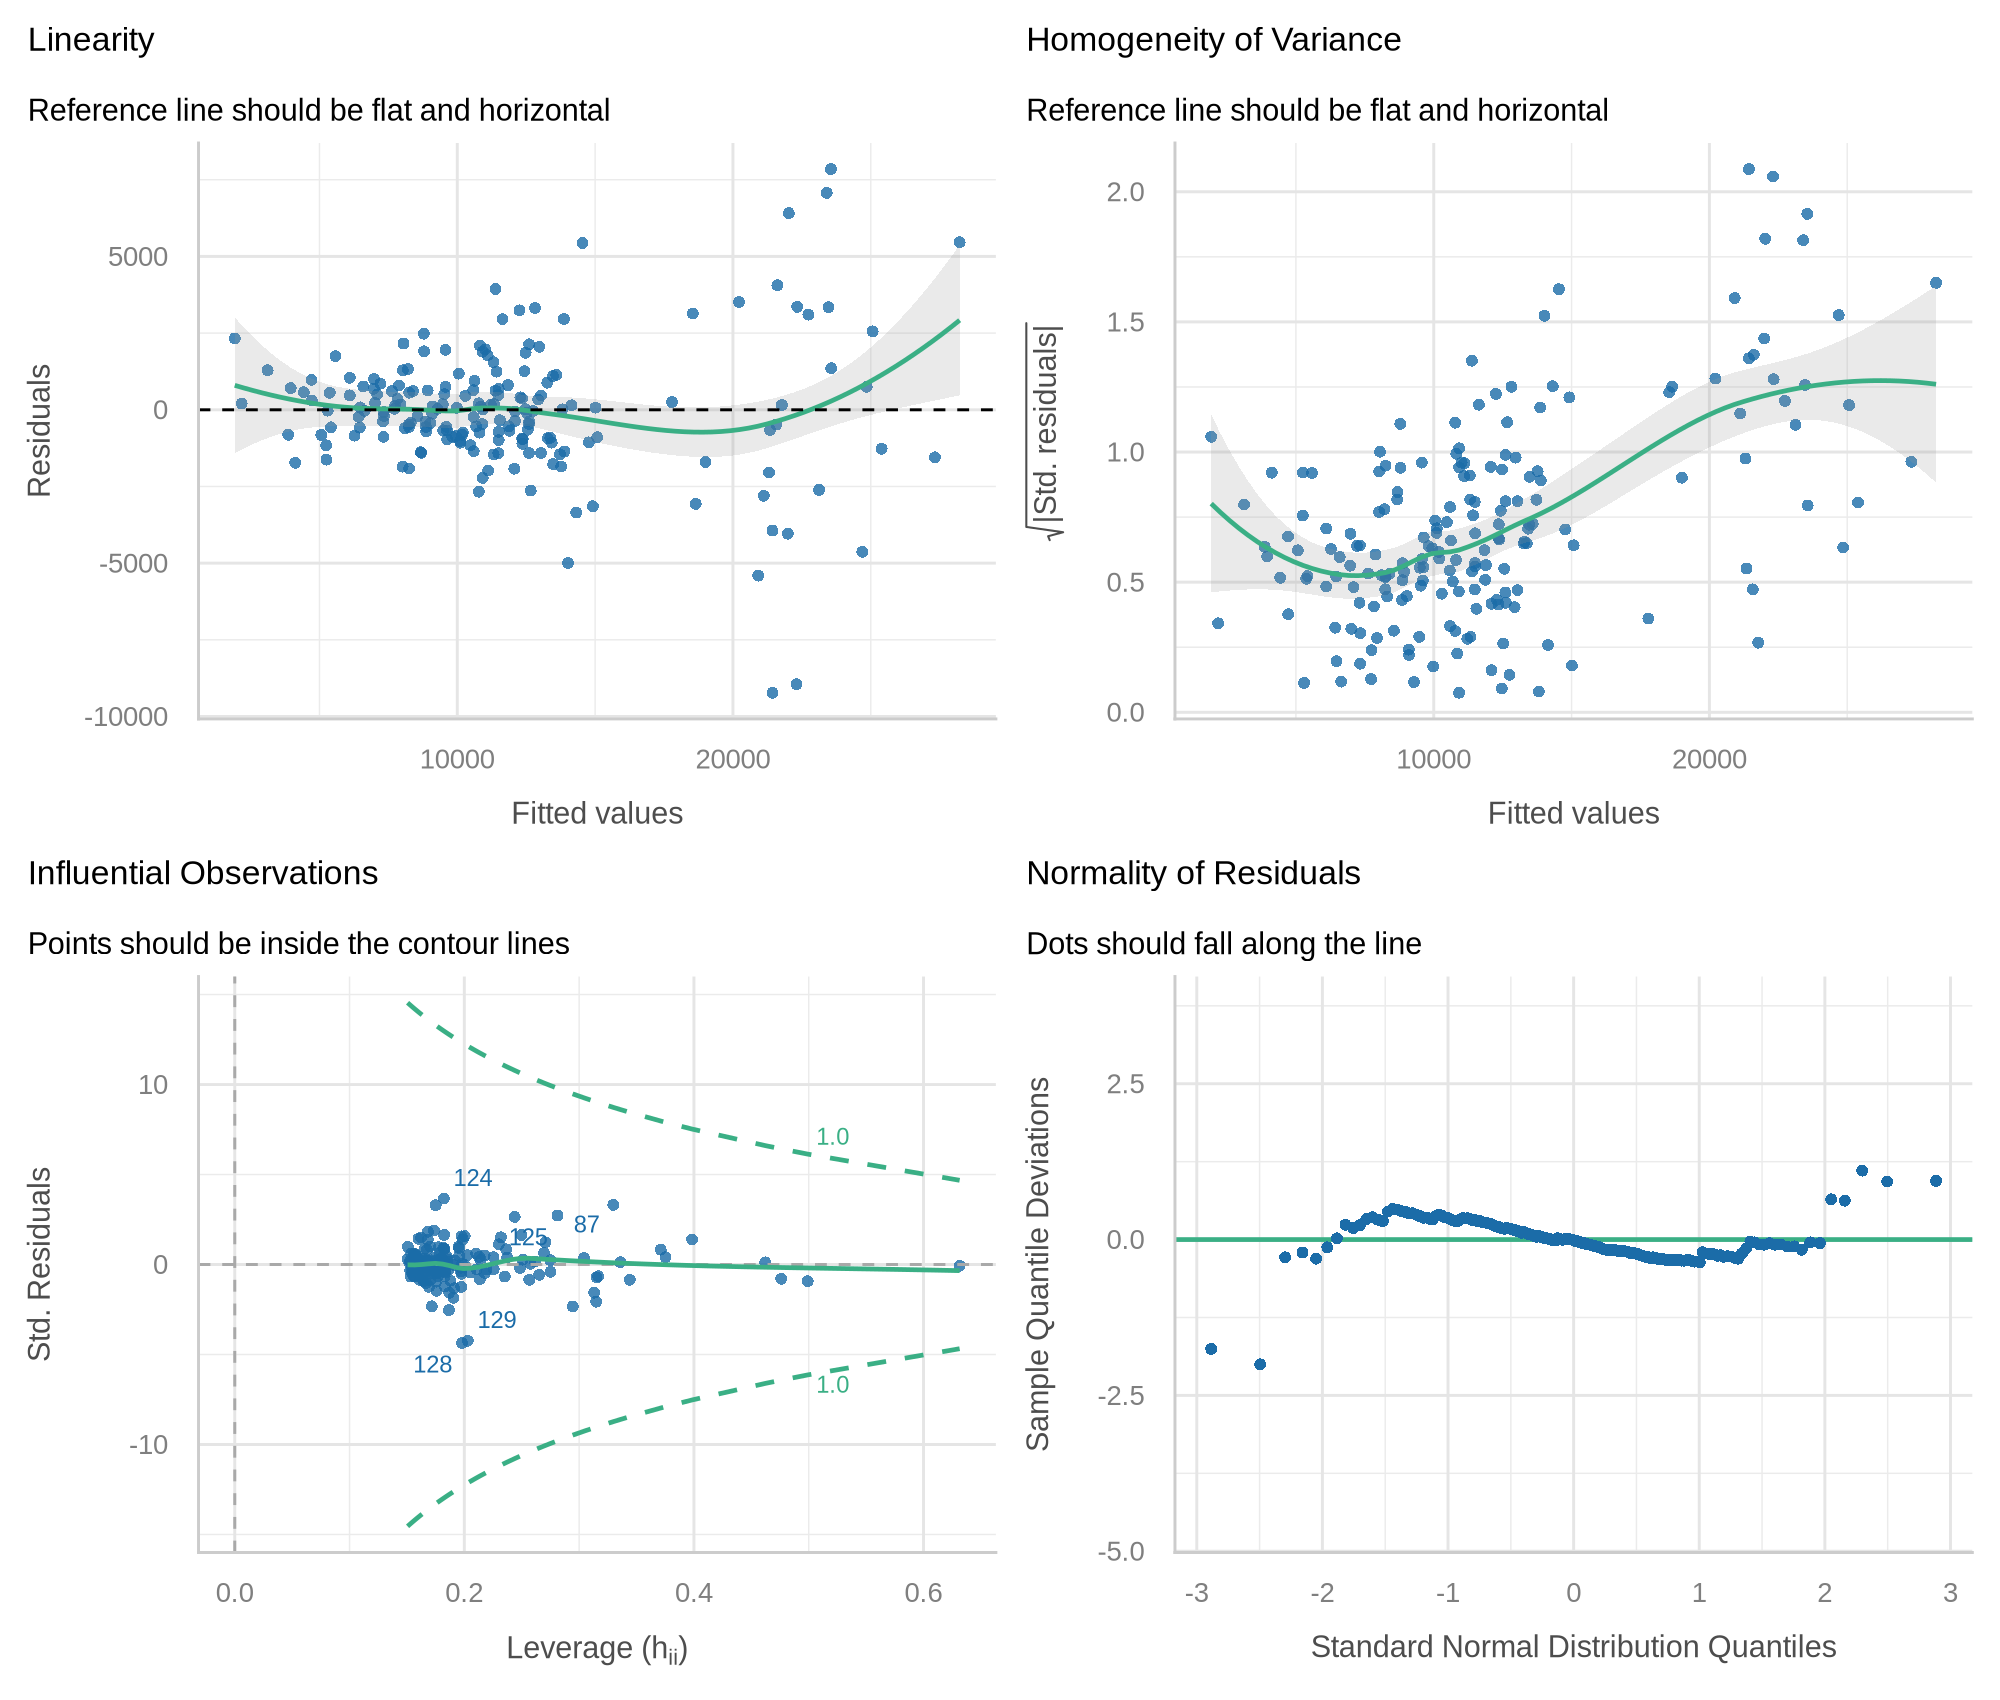
\includegraphics[width=0.8\textwidth]{r04_check_model.png}
\caption{Diagnóstico del modelo de efectos fijos con \code{performance::check\_model()}.}\label{fig:diag}
\end{figure}
\section{6. Rama 4: analítica predictiva (réplica del artículo)}
La rama 4 repite la validación walk-forward del artículo: en cada año de prueba (2021--2025) se entrena con los años anteriores y se pronostica un año adelante para los 19 departamentos, lo que da 95 pronósticos fuera de muestra. Se comparan seis modelos con los hiperparámetros fijados en el artículo. El Ridge se resolvió en forma cerrada y el ElasticNet por descenso de coordenadas con la función objetivo de scikit-learn; su solución se verificó con las condiciones de optimalidad KKT. El panel FE-ARDL se volvió a ajustar con \code{caret::train()} usando los mismos índices walk-forward y los pronósticos coincidieron exactamente.

\begin{table}[htbp]
\centering
\small
\caption{Desempeño fuera de muestra (95 pronósticos, 2021--2025) en R, frente al artículo de referencia. La última columna es la mayor diferencia absoluta (kg/ha) entre cada pronóstico y el de Python.}\label{tab:modelos}
\begin{tabular}{lrrrrrr}
\toprule
Modelo & MAE & RMSE & MAPE & MAE art. & RMSE art. & Dif. máx. \\
\midrule
Naive Lag1 & 2\,044.97 & 3\,361.84 & 17.43\,\% & 2\,044.97 & 3\,361.84 & 1.8e-12 \\
Panel FE-ARDL & 2\,601.96 & 3\,829.68 & 23.95\,\% & 2\,601.96 & 3\,829.68 & 1.7e-9 \\
Ridge & 2\,240.12 & 3\,346.52 & 22.11\,\% & 2\,240.12 & 3\,346.52 & 9.1e-12 \\
ElasticNet & 3\,694.59 & 5\,007.97 & 44.74\,\% & 3\,694.59 & 5\,007.97 & 3.0e-5 \\
XGBoost (prof. 2) & 2\,349.36 & 3\,300.15 & 25.60\,\% & 2\,349.36 & 3\,300.15 & 8.6e-4 \\
Ensamble informado & 2\,194.22 & 3\,092.66 & 21.10\,\% & 2\,194.22 & 3\,092.66 & 8.3e-10 \\
\bottomrule
\end{tabular}
\end{table}
Los cuatro modelos deterministas coinciden con Python hasta 2e-09 kg/ha (ElasticNet: 3.0e-05, por la tolerancia de scikit-learn). Con la misma semilla, \pkg{xgboost} 3.4.2.1 de R reprodujo también el XGBoost del artículo (diferencia máxima de 0.0009 kg/ha, del orden de la precisión de 32 bits), así que el cuadro coincide con el artículo en los seis modelos.

El ensamble reduce el RMSE en 8.0\,\% frente al ingenuo, pero no el MAE (2\,194.22 frente a 2\,044.97): comete menos errores grandes, aunque en los casos típicos el valor del año anterior sigue siendo difícil de superar. Al repetir el XGBoost con 10 semillas, el RMSE del ensamble queda entre 3\,037.34 y 3\,092.66 kg/ha y supera al ingenuo en 10 de 10 casos (Figura~\ref{fig:rvp}).

\begin{figure}[htbp]
\centering
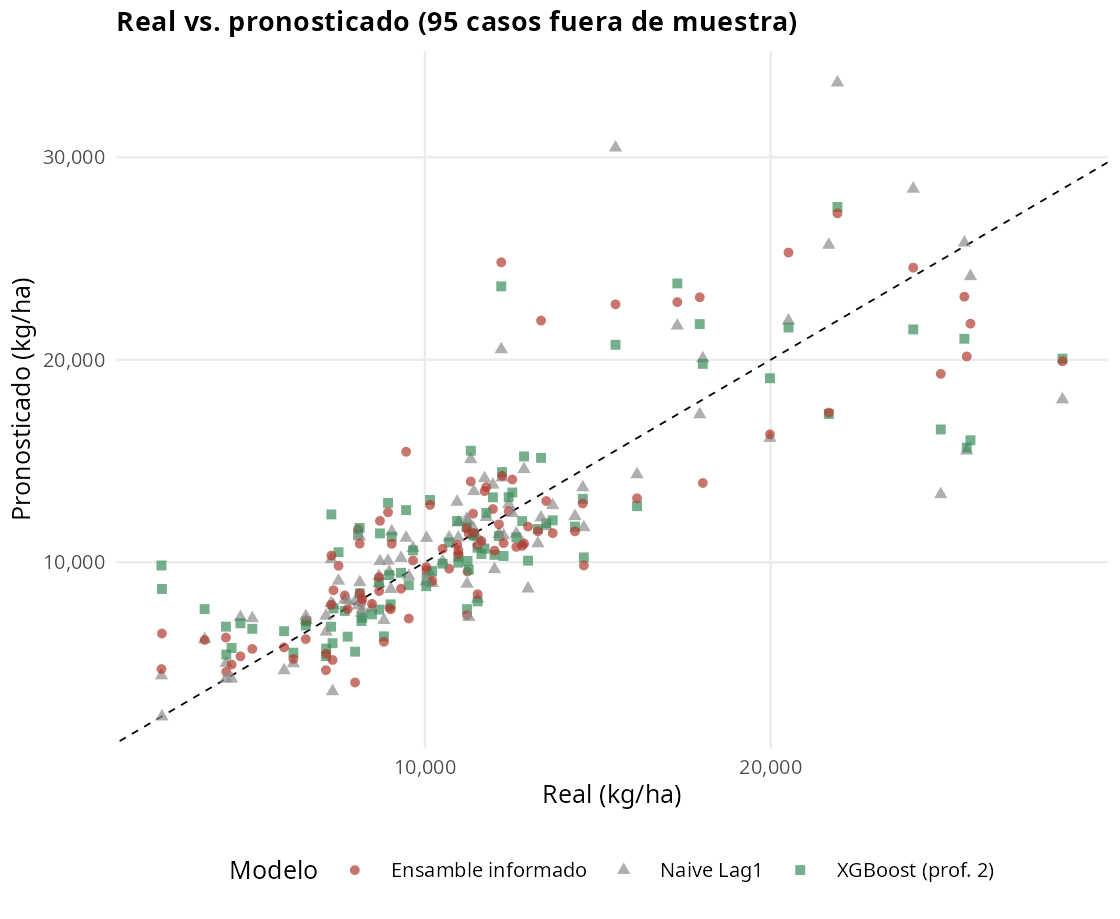
\includegraphics[width=0.55\textwidth]{r05_real_vs_pred.png}
\caption{Rendimiento real frente al pronosticado en los 95 casos de prueba.}\label{fig:rvp}
\end{figure}
La incertidumbre se calibra con split-conformal \citep{conformal}: el último año de cada ventana de entrenamiento se pronostica con los años previos y el cuantil $\lceil (n+1)(1-\alpha)\rceil/n$ de esos errores ($n=19$) da el ancho del intervalo.

\begin{Verbatim}[fontsize=\scriptsize, frame=single, framesep=2mm, label={\small Cuantil split-conformal}]
cuantil_conformal <- function(res_abs, nivel) {
\end{Verbatim}
\begin{table}[htbp]
\centering
\small
\caption{Intervalos de predicción del ensamble antes y después de la calibración split-conformal.}\label{tab:conf}
\begin{tabular}{lrrrrr}
\toprule
Nominal & Método & Cobertura & Error (pp) & Ancho medio & Winkler \\
\midrule
80 \% & Gaussiano (sin calibrar) & 50.5\,\% & -29.5 & 3\,298.7 & 14\,030.1 \\
80 \% & Split-conformal & 81.1\,\% & +1.1 & 7\,420.5 & 11\,481.8 \\
90 \% & Gaussiano (sin calibrar) & 58.9\,\% & -31.1 & 4\,233.8 & 21\,594.7 \\
90 \% & Split-conformal & 92.6\,\% & +2.6 & 10\,694.7 & 14\,416.3 \\
\bottomrule
\end{tabular}
\end{table}
Los intervalos gaussianos quedan muy cortos (50.5\,\% de cobertura al 80\,\% nominal); con calibración conformal la cobertura sube a 81.1\,\% y 92.6\,\% al 90\,\%, a cambio de intervalos más anchos (Figura~\ref{fig:conf}).

\begin{figure}[htbp]
\centering
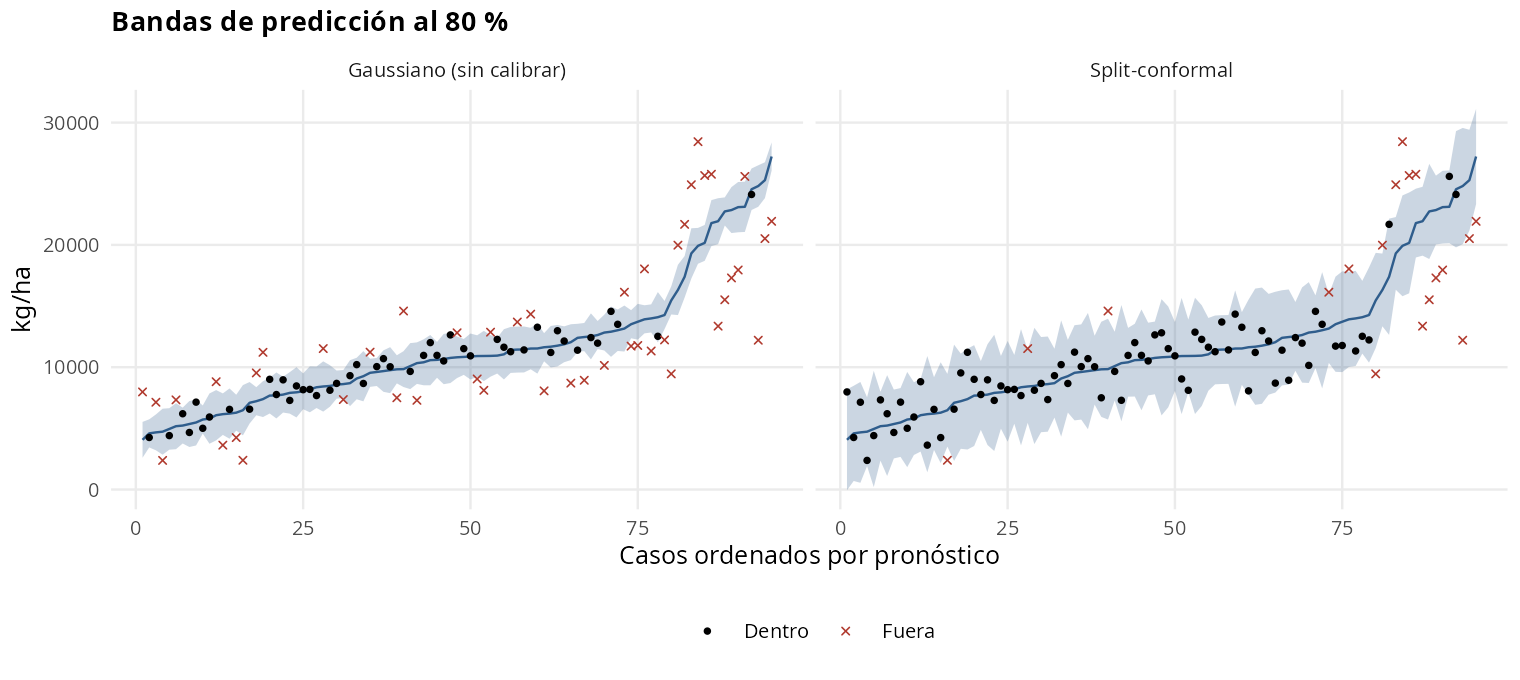
\includegraphics[width=\textwidth]{r06_conformal.png}
\caption{Bandas al 80\,\%: gaussiana (izquierda) y split-conformal (derecha).}\label{fig:conf}
\end{figure}
En los 33 casos con heladas en al menos 5\,\% de productores, el ensamble baja el MAE de 1\,880.04 a 1\,657.89 kg/ha y el RMSE de 2\,827.45 a 2\,268.53. El rendimiento del año previo domina la importancia SHAP \citep{shap} (2\,438 kg/ha de contribución media), seguido de riego, crédito, semilla cert., capacitación. Los residuos del ensamble tienen media -103 kg/ha y colas pesadas (Shapiro--Wilk $p = 0.002$), lo que respalda el uso de intervalos conformales (Figuras~\ref{fig:estab} y~\ref{fig:resh}).

\begin{table}[htbp]
\centering
\small
\caption{Sensibilidad del ensamble informado (kg/ha).}\label{tab:sens}
\begin{tabular}{lrrr}
\toprule
Escenario & MAE & RMSE & MAPE \\
\midrule
Base: ventana expansiva, 10 covariables, profundidad 2 & 2\,194.22 & 3\,092.66 & 21.10\,\% \\
Ventana móvil de 4 años & 2\,203.15 & 3\,192.66 & 20.47\,\% \\
Ventana móvil de 3 años & 2\,140.88 & 2\,964.98 & 20.42\,\% \\
XGBoost con profundidad 3 & 2\,219.35 & 3\,141.88 & 21.49\,\% \\
Sin covariables de pérdidas climáticas & 1\,972.55 & 2\,907.41 & 18.24\,\% \\
Solo riego, semilla y fertilizante & 2\,037.62 & 3\,016.35 & 20.41\,\% \\
\bottomrule
\end{tabular}
\end{table}
\begin{figure}[htbp]
\centering
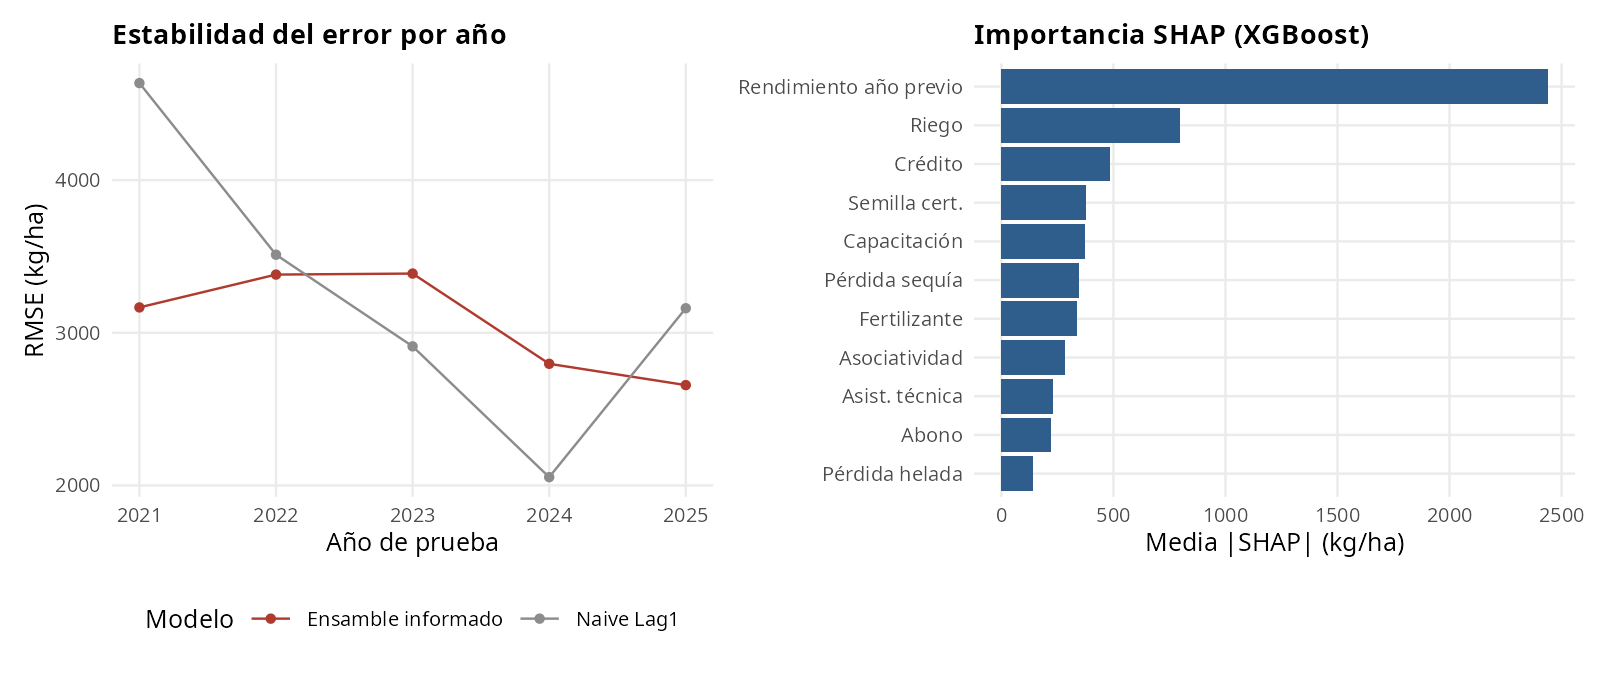
\includegraphics[width=\textwidth]{r07_estabilidad_shap.png}
\caption{RMSE por año de prueba e importancia SHAP del XGBoost.}\label{fig:estab}
\end{figure}
\begin{figure}[htbp]
\centering
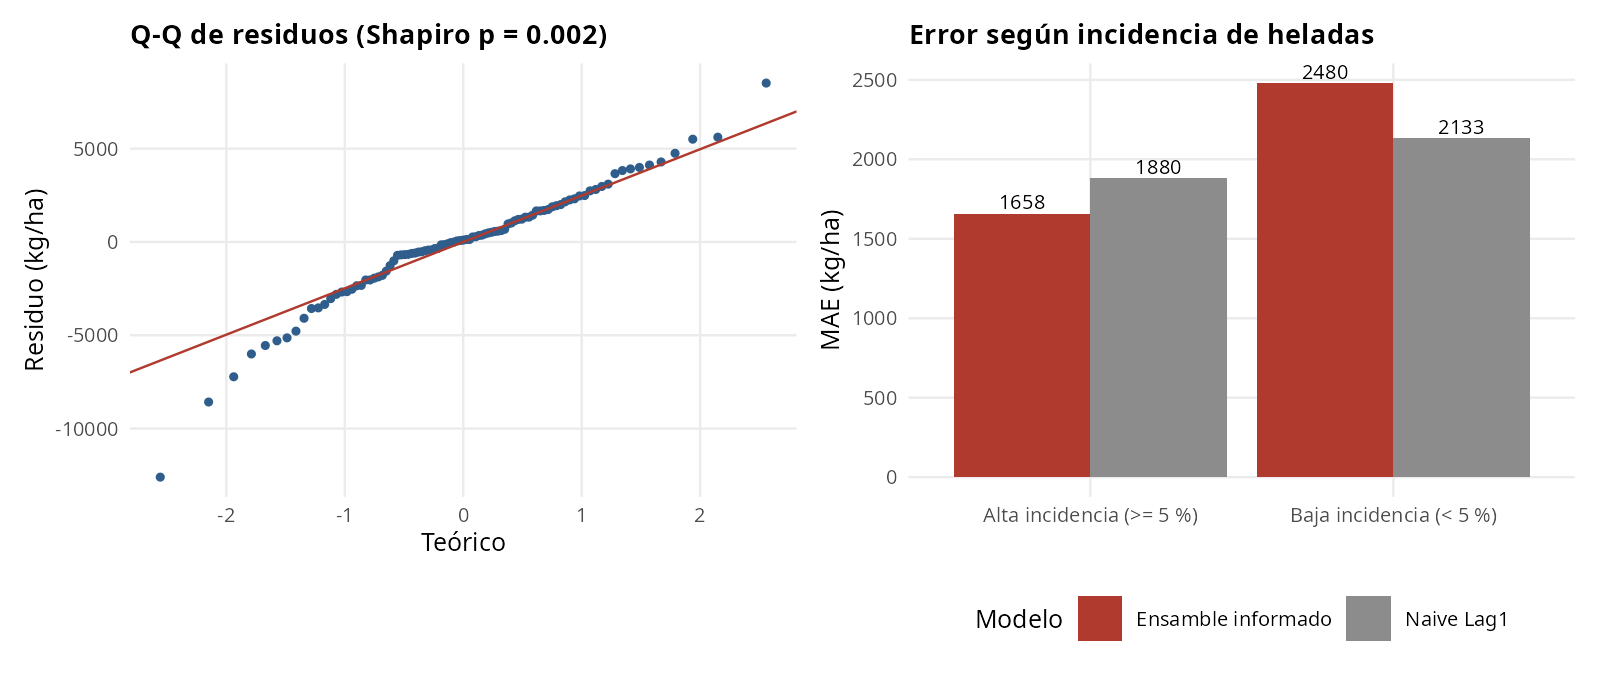
\includegraphics[width=\textwidth]{r08_residuos_heladas.png}
\caption{Residuos del ensamble y error según la incidencia de heladas.}\label{fig:resh}
\end{figure}
\section{7. Rama 5: analítica prescriptiva}
\subsection{7.1 Alerta temprana 2026 y departamentos priorizados}
El ensamble, entrenado con todos los años, pronostica 2026 suponiendo que las covariables se mantienen como en 2025, con un intervalo conformal al 80\,\% calibrado en 2025. Un departamento es \emph{priorizado} si tuvo heladas con pérdida total en al menos 5\,\% de productores en promedio entre 2021 y 2025 y, además, su pronóstico 2026 está por debajo de su media histórica o su rendimiento medio está bajo el promedio nacional. Resultan 6: Puno, Cusco, La Libertad, Huancavelica, Pasco, Apurímac (Figura~\ref{fig:ale}).

\begin{figure}[htbp]
\centering
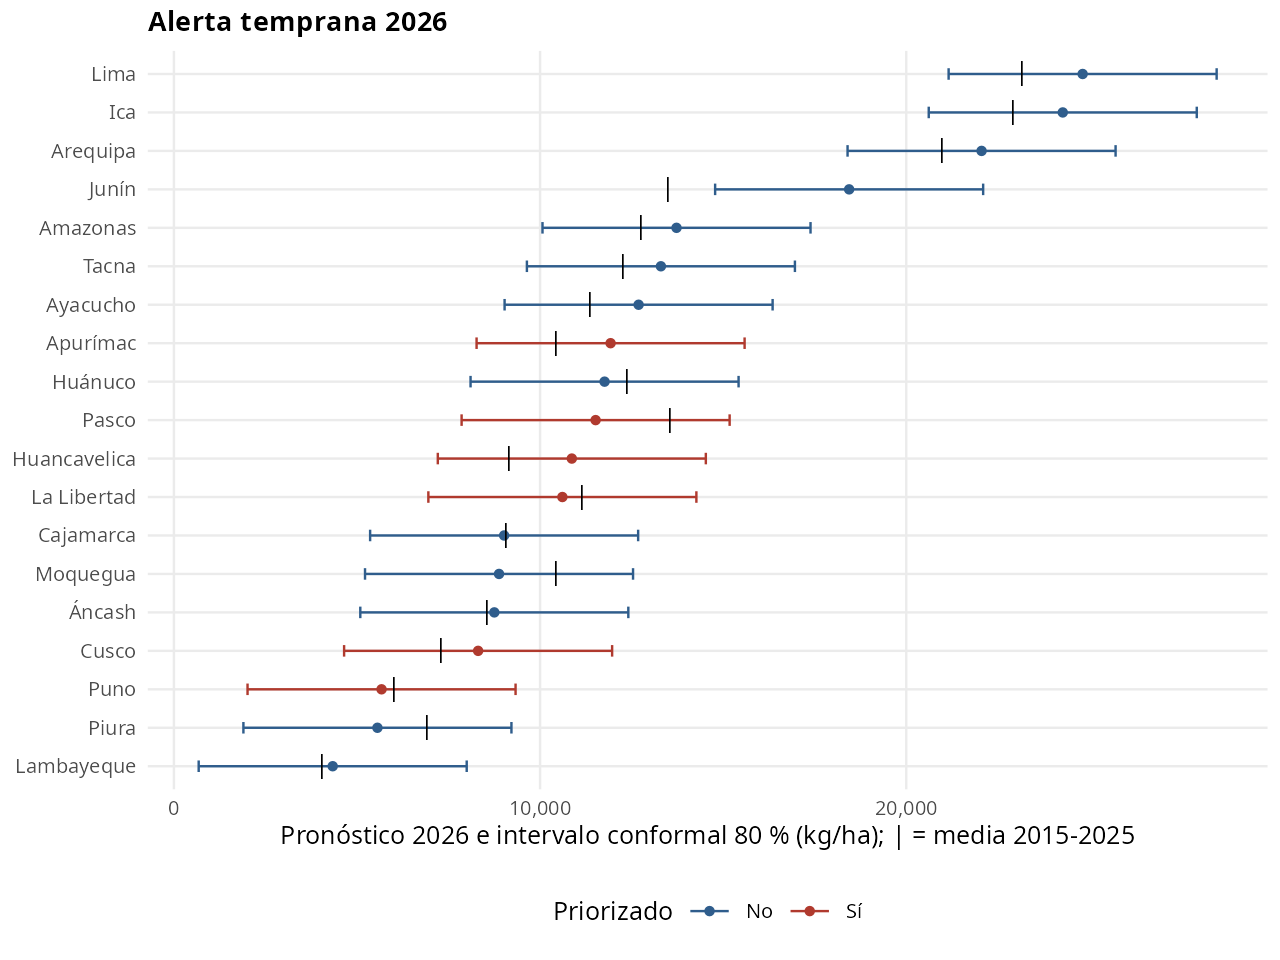
\includegraphics[width=0.75\textwidth]{r09_alerta_2026.png}
\caption{Pronóstico 2026 con intervalo conformal al 80\,\%. La marca vertical es la media 2015--2025.}\label{fig:ale}
\end{figure}
\subsection{7.2 Formulación}
Sea $x_{ik}$ el aumento, en puntos porcentuales, de la palanca $k$ en el departamento $i$. El programa lineal es
\begin{align*}
\max_{x}\; & \textstyle\sum_{i,k} \beta_k\, S_i\, p_i\, x_{ik} \\
\text{s.a.}\; & \textstyle\sum_{i,k} c_{ik}\, x_{ik} \le B, \qquad \sum_{k} c_{ik}\, x_{ik} \le 0.25\,B \;\; \forall i, \qquad \sum_{i \in P}\sum_k c_{ik}\, x_{ik} \ge 0.30\,B, \\
& 0 \le x_{ik} \le \min(\bar{x}_k,\, 100 - L_{ik}),
\end{align*}
donde $S_i$ es la superficie cosechada 2025 (ha), $p_i$ el precio de venta (S/ por kg), $L_{ik}$ el nivel actual de la palanca, $\bar{x}_k$ su tope por campaña, $P$ el conjunto priorizado y $c_{ik}$ el costo de subir un punto ($c_k S_i/100$ para palancas por área y $c_k N_i/100$ para palancas por productor, con $N_i$ productores). Se resuelven dos versiones: con $\beta$ puntual y con $\beta$ robusto, la cota inferior al 80\,\%. Los costos unitarios son supuestos razonables que el tablero permite cambiar (Cuadro~\ref{tab:palancas}).

\begin{table}[htbp]
\centering
\small
\caption{Palancas de decisión: efecto por punto porcentual (kg/ha), efecto robusto $\max(0,\hat\beta-1.28\,\mathrm{EE})$, costo unitario por campaña y aumento máximo.}\label{tab:palancas}
\begin{tabular}{lrrrrr}
\toprule
Palanca & $\beta$ puntual & EE & $\beta$ robusto & Costo (S/, supuesto) & Tope (pp) \\
\midrule
Riego tecnificado & 4.1 & 29.0 & 0.0 & 1\,500 por ha & 10 \\
Semilla certificada & 70.5 & 18.0 & 47.4 & 3\,000 por ha & 10 \\
Asistencia técnica & 101.0 & 65.8 & 16.7 & 600 por productor & 15 \\
Crédito agrario & 43.7 & 52.5 & 0.0 & 500 por productor & 10 \\
\bottomrule
\end{tabular}
\end{table}
\begin{Verbatim}[fontsize=\scriptsize, frame=single, framesep=2mm, label={\small Programa lineal con lpSolve}]
optimizar_plan <- function(insumos, palancas, efectos, presupuesto, cuota = CUOTA_EQUIDAD,
                           tope_depto = TOPE_DEPTO, tipo = "puntual") {
  pr <- armar_problema(insumos, palancas, efectos, tipo)
  n <- nrow(pr)
  if (n == 0) stop("Ninguna palanca tiene efecto positivo: no hay plan que optimizar")
  deps <- unique(pr$DEPARTAMENTO)
  # capacidad de los priorizados: si no alcanza la cuota, la cuota se ajusta a su capacidad
  cap_prior <- sum((pr$c * pr$ub)[pr$prioritario])
  rhs_eq <- min(cuota * presupuesto, cap_prior)
  A <- rbind(pr$c,
             t(vapply(deps, function(d) pr$c * (pr$DEPARTAMENTO == d), numeric(n))),
             pr$c * pr$prioritario,
             diag(n))
  dir <- c("<=", rep("<=", length(deps)), ">=", rep("<=", n))
  rhs <- c(presupuesto, rep(tope_depto * presupuesto, length(deps)), rhs_eq, pr$ub)
  sol <- lpSolve::lp("max", pr$v, A, dir, rhs, compute.sens = TRUE)
  if (sol$status != 0) stop("El programa lineal no tiene solución (status ", sol$status, ")")
  pr$x <- sol$solution
  pr <- mutate(pr, costo = c * x, kg_adic = kg * x, valor = v * x)
  list(plan = pr, objetivo = sol$objval, gasto = sum(pr$costo),
       precio_sombra = sol$duals[1],      # S/ adicionales por cada sol extra de presupuesto
       cuota_efectiva = rhs_eq / presupuesto, cap_prior = cap_prior, status = sol$status)
}
\end{Verbatim}
\subsection{7.3 Resultados}
El plan puntual concentra el gasto en asistencia técnica y crédito y promete S/ 509.8 millones de valor adicional (beneficio/costo 10.2). Esa cifra descansa en coeficientes imprecisos. El plan robusto descarta las palancas cuyo efecto no se distingue de cero (riego y crédito) y pone S/ 41.5 millones en semilla certificada y S/ 8.5 millones en asistencia técnica (Cuadro~\ref{tab:plan}, Figura~\ref{fig:plan}). Rinde S/ 131.7 millones (83\,255 t adicionales) aun con efectos conservadores, y el 65\,\% del presupuesto va a departamentos priorizados.

\begin{table}[htbp]
\centering
\footnotesize
\caption{Plan robusto recomendado para un presupuesto de S/ 50 millones por campaña.}\label{tab:plan}
\begin{tabular}{llrrrc}
\toprule
Departamento & Palanca(s) & S/ M & t adicionales & Valor S/ M & Prior. \\
\midrule
Cusco & Semilla certificada & 10.22 & 16\,136 & 24.01 & sí \\
La Libertad & Asistencia técnica, Semilla certificada & 9.33 & 14\,874 & 24.17 & sí \\
Puno & Semilla certificada & 8.00 & 12\,634 & 26.42 & sí \\
Cajamarca & Semilla certificada & 7.74 & 12\,214 & 18.37 &  \\
Huancavelica & Semilla certificada & 5.02 & 7\,931 & 11.40 & sí \\
Ayacucho & Asistencia técnica & 3.83 & 7\,732 & 9.28 &  \\
Lima & Asistencia técnica, Semilla certificada & 3.34 & 6\,142 & 10.19 &  \\
Áncash & Semilla certificada & 0.82 & 1\,289 & 1.79 &  \\
Moquegua & Semilla certificada & 0.67 & 1\,056 & 1.96 &  \\
Amazonas & Asistencia técnica & 0.54 & 1\,250 & 1.65 &  \\
Tacna & Semilla certificada & 0.36 & 566 & 1.16 &  \\
Ica & Asistencia técnica & 0.14 & 1\,432 & 1.34 &  \\
\bottomrule
\end{tabular}
\end{table}
\begin{figure}[htbp]
\centering
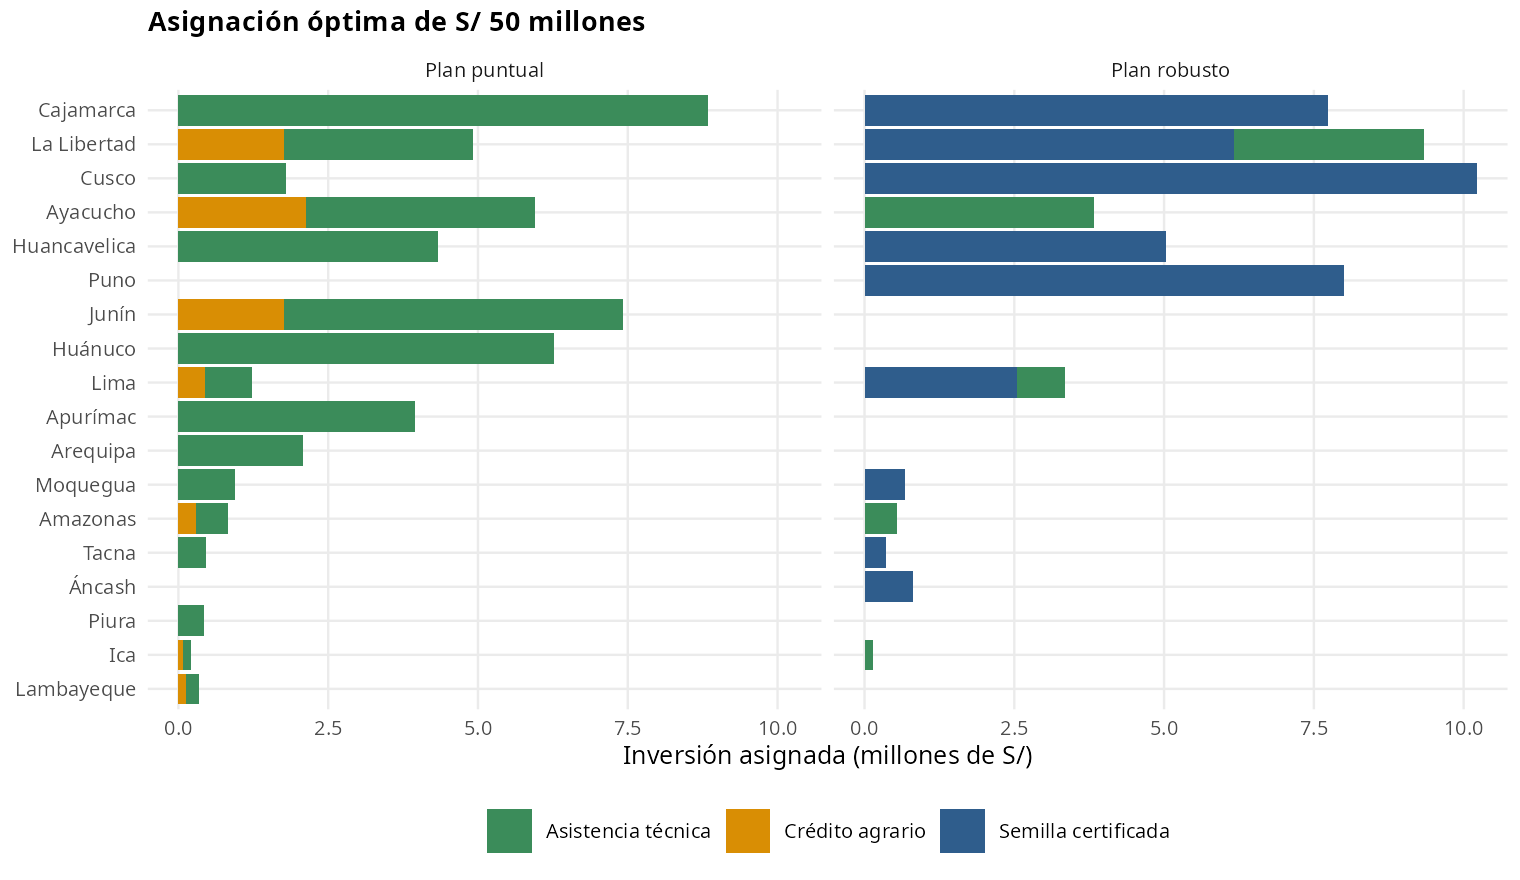
\includegraphics[width=\textwidth]{r10_plan_optimo.png}
\caption{Asignación óptima de S/ 50 millones con efectos puntuales (izquierda) y robustos (derecha).}\label{fig:plan}
\end{figure}
El Cuadro~\ref{tab:mc} evalúa ambos planes cuando el efecto verdadero varía según su incertidumbre. El plan puntual tiene mayor valor esperado, pero su peor 5\,\% cae a S/ 83.4 millones y la probabilidad de no recuperar la inversión es 3.81\,\%. El plan robusto tiene un peor 5\,\% más alto (S/ 138.8 millones) y esa probabilidad baja a 0.59\,\%. Para una entidad pública que debe rendir cuentas, el plan robusto es la recomendación.

\begin{table}[htbp]
\centering
\small
\caption{Valor de cada plan (millones de S/) cuando el efecto verdadero varía según la incertidumbre estimada (normal multivariada con la covarianza agrupada). Las columnas exactas usan la normalidad del valor; la última viene de 20\,000 simulaciones.}\label{tab:mc}
\begin{tabular}{lrrrrr}
\toprule
Plan & Valor esperado & P05 & P95 & P(B/C $<$ 1) & P05 Montecarlo \\
\midrule
Plan puntual & 509.8 & 83.4 & 936.2 & 3.81\,\% & 79.0 \\
Plan robusto & 306.3 & 138.8 & 473.8 & 0.59\,\% & 137.6 \\
\bottomrule
\end{tabular}
\end{table}
La frontera de la Figura~\ref{fig:front} muestra cuánto presupuesto vale la pena. Con S/ 50 millones, un sol adicional rinde S/ 2.20 en el plan robusto (precio sombra). Con efectos robustos, cada sol extra sigue rindiendo más de un sol hasta S/ 130 millones; por encima de esa cifra conviene buscar otras palancas. La capacidad total del plan robusto se agota en S/ 172.6 millones. La cuota de equidad del 30\,\% cuesta S/ 0.31 millones en el plan puntual y una cuota del 50\,\% costaría S/ 7.9 millones: proteger a los departamentos con heladas sale barato. Si los costos unitarios fueran 50\,\% menores o mayores, el beneficio/costo del plan puntual iría de 8.0 a 15.4; la recomendación no cambia de signo.

\begin{figure}[htbp]
\centering
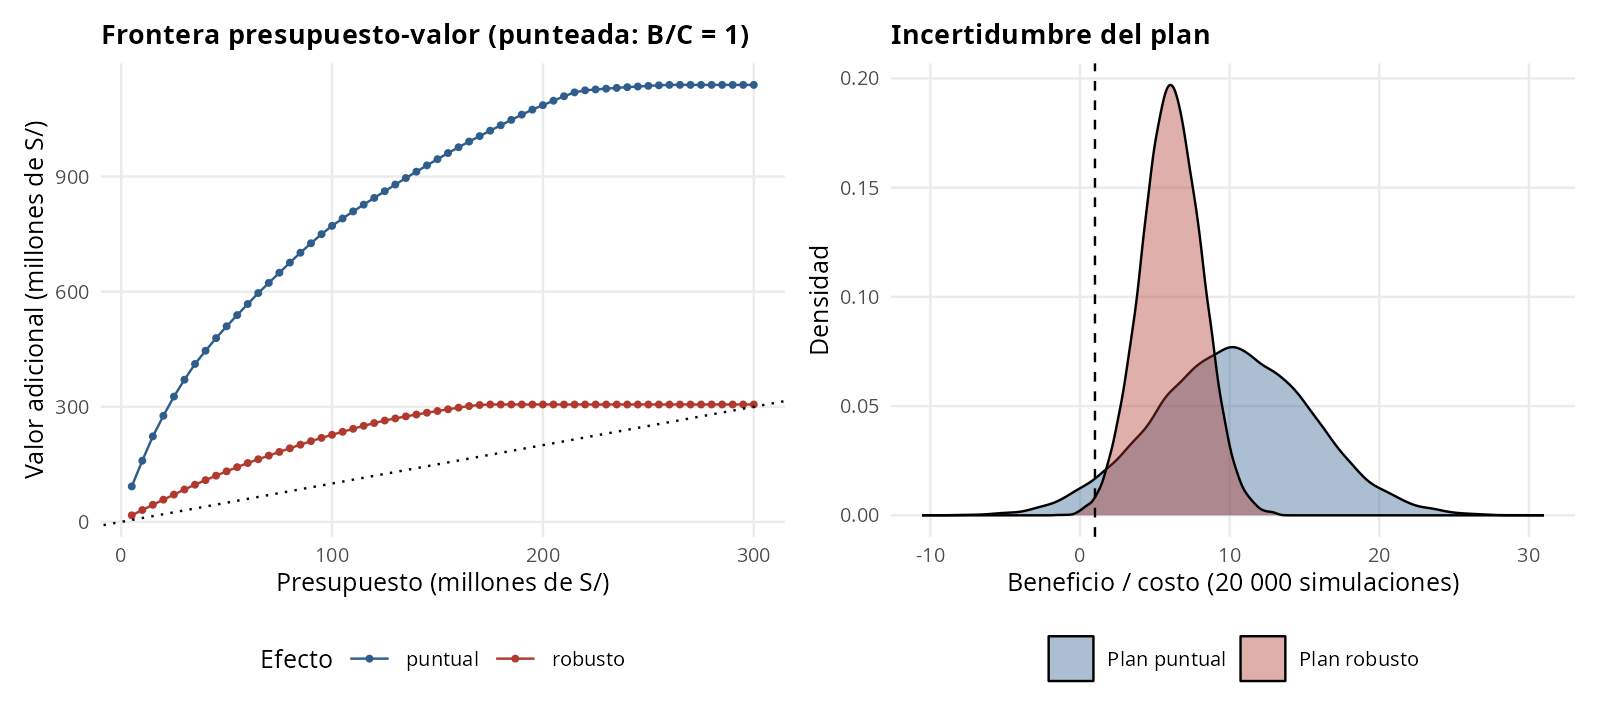
\includegraphics[width=\textwidth]{r11_frontera_montecarlo.png}
\caption{Frontera presupuesto--valor y distribución del beneficio/costo de cada plan.}\label{fig:front}
\end{figure}
\section{8. Rama 6: comunicación y pruebas}
Un resultado que nadie entiende no se usa. El tablero \pkg{shiny} (Figura~\ref{fig:shiny}) deja al usuario mover el presupuesto, el tipo de efecto, la cuota de equidad, el tope por departamento y los costos unitarios; el programa lineal se resuelve en vivo y muestra cuatro indicadores: valor adicional, producción adicional, beneficio/costo y el valor de un sol extra. La lógica del servidor se prueba con \code{shiny::testServer()} y la aplicación completa con \pkg{shinytest2} en Chrome; las funciones del pipeline tienen pruebas \pkg{testthat} con casos de solución conocida (por ejemplo, un programa lineal de dos departamentos que se resuelve a mano).

\begin{figure}[htbp]
\centering
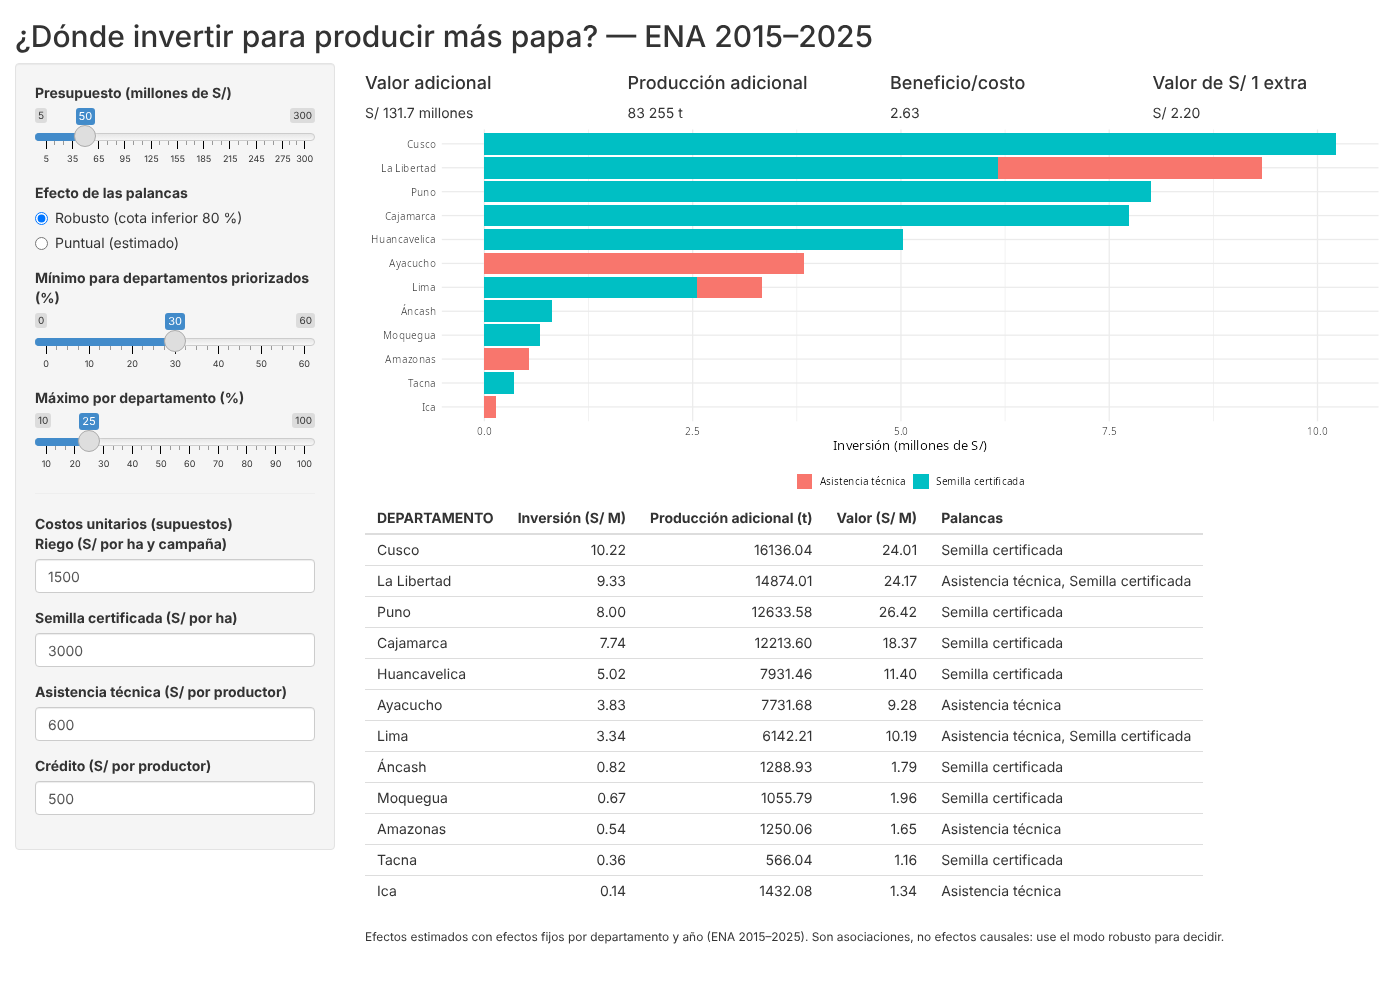
\includegraphics[width=0.92\textwidth]{r12_tablero_shiny.png}
\caption{Tablero \pkg{shiny}: plan robusto con S/ 50 millones.}\label{fig:shiny}
\end{figure}
\section{9. Resumen de validaciones}
El pipeline en R ejecutó 61 validaciones y todas fueron aprobadas (Cuadro~\ref{tab:val}). El registro completo está en el archivo \code{registro\_validaciones.csv} de la carpeta de tablas.

\begin{table}[htbp]
\centering
\small
\caption{Validaciones automáticas del pipeline en R (el pipeline se detiene si alguna falla).}\label{tab:val}
\begin{tabular}{lrr}
\toprule
Rama & Validaciones & Aprobadas \\
\midrule
Datos & 22 & 22 \\
Descriptivo & 4 & 4 \\
Predictivo & 15 & 15 \\
Prescriptivo & 19 & 19 \\
Comunicación & 1 & 1 \\
\bottomrule
\end{tabular}
\end{table}
\section{10. Conclusiones}
\begin{enumerate}
\item El panel se reconstruyó desde los microdatos sin diferencias con el Excel, y los seis modelos del artículo se reprodujeron en R.
\item El ensamble informado tiene el menor RMSE (3\,092.66 kg/ha) y la calibración conformal es indispensable: sin ella los intervalos cubren la mitad de lo que prometen.
\item Con S/ 50 millones, el plan robusto invierte sobre todo en semilla certificada en Cusco, Puno, Cajamarca, Huancavelica y La Libertad, y en asistencia técnica donde hay más superficie por productor. Produce 83\,255 t adicionales y un beneficio/costo de 2.63 con efectos conservadores.
\item Hasta S/ 130 millones cada sol adicional rinde más de un sol; la cuota de equidad para los departamentos con heladas cuesta menos del 1\,\% del valor.
\end{enumerate}

\textbf{Limitaciones.} Los efectos vienen de un panel observacional de diez años: son asociaciones dentro de cada departamento, no efectos causales, y suponen que se mantienen al escalar la intervención. Los costos unitarios son supuestos; el tablero y el análisis de sensibilidad muestran cómo cambia el plan si se ajustan. El pronóstico 2026 supone covariables iguales a 2025 y no incluye clima directo (temperatura o precipitación).

\section{Anexo: cómo ejecutar}
\begin{Verbatim}[fontsize=\scriptsize, frame=single, framesep=2mm, label={\small Comandos}]
# desde la raíz del proyecto (o abrir ENA_papa_prescriptivo.Rproj en RStudio)
Rscript R/run_all.R
# tablero
Rscript -e 'shiny::runApp("R/app")'
# pruebas
Rscript -e 'testthat::test_dir("R/tests")'
\end{Verbatim}

\begin{thebibliography}{99}

\bibitem[Bezanson et~al.(2017)]{julia} Bezanson, J., Edelman, A., Karpinski, S. y Shah, V. B. (2017). Julia: A fresh approach to numerical computing. \emph{SIAM Review}, 59(1), 65--98.

\bibitem[Callohuanca et~al.(2026)]{articulo} Callohuanca Condori, D. L., Mamani Huatta, C. D., Gomez Cahuana, J. R., Mamani Emanuel, E. W. y Rosas Tuni, R. C. (2026). \emph{Pronóstico del rendimiento de papa en el Perú con historial reducido}. Ciencia de Datos I, FINESI-UNA Puno.

\bibitem[Chen y Guestrin(2016)]{xgboost} Chen, T. y Guestrin, C. (2016). XGBoost: A scalable tree boosting system. En \emph{Proceedings of KDD 2016}, 785--794.

\bibitem[Dunning et~al.(2017)]{jump} Dunning, I., Huchette, J. y Lubin, M. (2017). JuMP: A modeling language for mathematical optimization. \emph{SIAM Review}, 59(2), 295--320.

\bibitem[Huang et~al.(2027)]{huang} Huang, R., Luo, W., Jiang, Y. et~al. (2027). A domain-informed forecasting framework for short-horizon carbon emissions prediction in power plants under reduced-history conditions. \emph{Electric Power Systems Research}, 265, 114351.

\bibitem[Huangfu y Hall(2018)]{highs} Huangfu, Q. y Hall, J. A. J. (2018). Parallelizing the dual revised simplex method. \emph{Mathematical Programming Computation}, 10(1), 119--142.

\bibitem[INEI(2025)]{inei} INEI (2025). \emph{Encuesta Nacional Agropecuaria (ENA) 2014--2024 y 2025, microdatos}. Lima: Instituto Nacional de Estadística e Informática.

\bibitem[Kuhn(2008)]{caret} Kuhn, M. (2008). Building predictive models in R using the caret package. \emph{Journal of Statistical Software}, 28(5), 1--26.

\bibitem[Lüdecke et~al.(2022)]{easystats} Lüdecke, D., Ben-Shachar, M. S., Patil, I. y Makowski, D. (2022). easystats: Framework for easy statistical modeling, visualization, and reporting. CRAN.

\bibitem[Lundberg y Lee(2017)]{shap} Lundberg, S. M. y Lee, S.-I. (2017). A unified approach to interpreting model predictions. En \emph{NeurIPS 30}, 4765--4774.

\bibitem[Vovk et~al.(2005)]{conformal} Vovk, V., Gammerman, A. y Shafer, G. (2005). \emph{Algorithmic Learning in a Random World}. Springer.

\bibitem[Wickham et~al.(2019)]{tidyverse} Wickham, H. et~al. (2019). Welcome to the tidyverse. \emph{Journal of Open Source Software}, 4(43), 1686.
\end{thebibliography}

\par\address{Rodrigo Claudio Rosas Tuni\\ Facultad de Ingeniería Estadística e Informática (FINESI)\\ Universidad Nacional del Altiplano, Puno, Perú}
\end{article}
\end{document}
